  
\chapter{MARCO CONCEPTUAL}

%=====================================
\section{VLAN}
\begin{definicion}[]
{
Una VLAN (Red de \'area local virtual o LAN virtual) es una red de \'area local que agrupa un conjunto de equipos de manera l\'ogica y no f\'isica. Efectivamente, la comunicaci\'on entre los diferentes equipos en una red de \'area local est\'a regida por la arquitectura f\'isica.
}
\end{definicion}lan 

\section{TIPOS VLAN}
\subsection{Puerto}
\begin{definicion}[]
{
Tambi\'en conocida como Port Switching en los men\'us de configuraci\'on de los routers y switches, se trata de la m\'as extendida y utilizada. Cada puerto se asigna a una VLAN y los usuarios que est\'en conectados a ese puerto pertenecen a la VLAN asignada. Los usuarios dentro de una misma VLAN poseen de visibilidad los unos sobre los otros, aunque no a las redes virtuales vecinas. El \'unico inconveniente es que no permite dinamismo a la hora de ubicar los usuarios y en el caso de que el usuario cambie de emplazamiento f\'isicamente se deber\'ia reconfigurar la red virtual.
}
\end{definicion}

\begin{caja}[]{
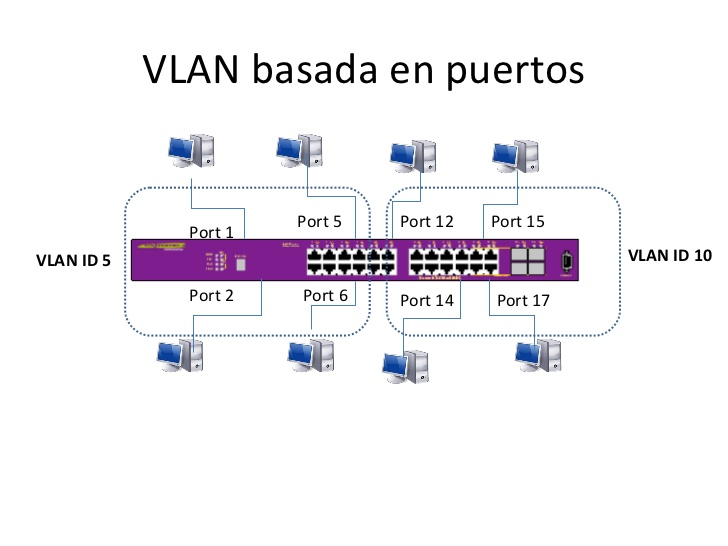
\includegraphics[scale=0.5]{img/puerto.jpg} 
 }\end{caja}
 Al inicio la vlan asignada por defecto es la vlan 1 por ello no es recomendado asignar esta vlan a una red.\\
 Cada puerto puede ser asignado a un vlan.\\

 \subsection{MAC}
 \begin{definicion}[]
{
 El razonamiento es similar a la anterior, salvo que en vez de ser una asignaci\'on a nivel de puerto lo es a nivel de direcci\'on MAC del dispositivo. La ventaja es que permite movilidad sin necesidad de que se tengan que aplicar cambios en la configuraci\'on del switch o del router. El problema parece bastante claro: a\~nadir todos los usuarios puede resultar tedioso.
}
\end{definicion}

\begin{caja}[]{
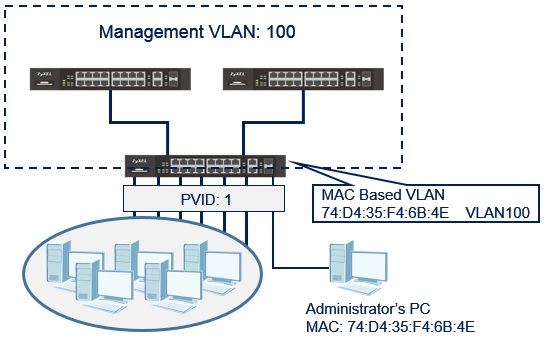
\includegraphics[scale=1]{img/mac.jpg} 
 }\end{caja}

 \subsection{Aplicaciones}
 \begin{definicion}[]
{
Se asignar\'ian redes virtuales en funci\'on de la aplicaci\'on utilizada, y en este caso intervienen varios factores, como por ejemplo la hora en la que nos encontramos, la direcci\'on MAC o la subred, permitiendo distinguir entre aplicaciones SSH, FTP, Samba o incluso SMTP.
}
\end{definicion}

\begin{caja}[]{
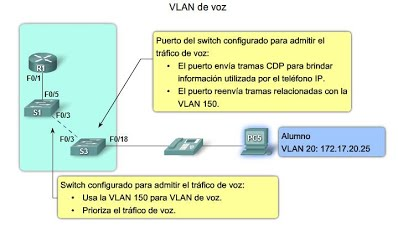
\includegraphics[scale=1]{img/aplicaciones.jpg} 
 }\end{caja}
